\section{Cross-VLM ranking inversion}
\label{sec:inversion}

If the strict-vs-semantic gap were a universal measurement-protocol artifact, it should affect all VLMs identically and preserve their relative rankings. We show this is false: two state-of-the-art open document VLMs reverse positions on the same evaluation under the two metrics, and two more architectures sign-flip the effect.

\paragraph{Head-to-head inversion (held-out and population scale).}
We re-run InternVL-2.5-8B on the same 358-row MTVQA held-out, judge with the same Gemini-Flash prompt, and restrict to the 353 rows for which both VLMs received a clean verdict (Table~\ref{tab:vlm-inversion}). Under strict-EM, InternVL leads by $9.6$ pp; under semantic-EM-C, Qwen leads by $6.8$ pp --- a $16.4$ pp swing in measured advantage attributable purely to metric choice. Across 2000 paired bootstrap resamples the joint inversion holds in $99.1\%$. We then re-judge both VLMs on the entire 9-language MTVQA val (intersection $n=2142$): Qwen strict $29.18\%$ vs InternVL $34.69\%$ (gap $-5.52$ pp, CI [$-7.47$, $-3.50$]); Qwen sem-C $60.55\%$ vs InternVL $48.60\%$ (gap $+11.95$ pp, CI [$+9.57$, $+14.24$]). \textbf{The inversion replicates at population scale with $P(\text{joint inversion}) = 1.000$.} The cross-VLM artifact-share split becomes significant at population: Qwen $+33.7\%$ [$+13.8$, $+52.8$] vs InternVL $+6.3\%$ [$-12.4$, $+24.2$], difference $+27.4$ pp [$+4.9$, $+51.0$]. Italian, Russian, and Korean show the largest single-language Qwen-over-InternVL sem-C gaps ($+18.5$, $+35.4$, $+16.6$ pp; Appendix~\ref{app:per-language-fullval-joint}).

\begin{table}[t]
\centering
\small
\begin{tabular}{lrr}
\toprule
metric & Qwen-7B & InternVL-8B \\
\midrule
strict-EM     & 24.4 \footnotesize{[19.8, 28.9]} & \textbf{34.0} \footnotesize{[29.2, 39.1]} \\
semantic-EM-C & \textbf{55.2} \footnotesize{[50.1, 60.6]} & 48.4 \footnotesize{[43.3, 54.1]} \\
\midrule
gap (Q$-$I) strict & \multicolumn{2}{r}{$-9.6$ pp \footnotesize{[$-14.2$, $-5.4$]}} \\
gap (Q$-$I) sem-C  & \multicolumn{2}{r}{$+6.8$ pp \footnotesize{[$+1.1$, $+12.2$]}} \\
\bottomrule
\end{tabular}
\caption{\textbf{Cross-VLM ranking inversion}, 353-row jointly-judged MTVQA held-out (\%). Brackets are 95\% percentile bootstrap CIs ($N=2000$). Both gaps exclude zero; the inversion is significant.}
\label{tab:vlm-inversion}
\end{table}

\paragraph{Cross-judge robustness.}
We re-run the same 716 (image, question, gold, prediction) tuples through \textbf{Gemini-2.5-Pro} using the identical prompt: 3-way Flash-vs-Pro agreement is $89.2\%$ on both VLMs ($\kappa = 0.819$/$0.827$), and the ranking inversion is preserved (Pro reports Qwen sem-C $52.6\%$ vs InternVL $48.0\%$; both judges agree on direction and approximate magnitude). The inversion claim is robust to judge identity. Full $3\times 3$ confusion in Appendix~\ref{app:judge-reliability}.

\paragraph{Inversion is not a single-pair effect: $2/6$ pairs invert.}
Across all six pairs in $\{\text{Qwen-7B}, \text{InternVL-8B}, \text{Phi-3.5}, \text{Llama-3.2-V-11B}\}$ on the held-out (paired bootstrap, $N{=}2000$), \textbf{two pairs invert}: Qwen vs InternVL ($P(\text{inv}){=}0.987$, the headline case above) and \textbf{Phi vs Llama} ($P(\text{inv}){=}0.887$): Phi leads on strict-EM by $+2.4$ pp [$-1.5$, $+6.0$], but Llama leads on semantic-EM-C by $+14.6$ pp [$+9.2$, $+19.9$]. The other four pairs (Qwen-vs-Phi, Qwen-vs-Llama, InternVL-vs-Phi, InternVL-vs-Llama) all compare a high-capability VLM against a low-capability one; both metrics correctly rank the stronger model first ($P(\text{inv}) \leq 0.001$). The inversion pattern is selective: it appears \emph{between models of similar capability with different output-style priors}, and disappears across capability gaps. This is the predicted shape of an output-style measurement artifact, not a universal protocol-noise effect.

\paragraph{Architecture-dependent artifact share.}
The script-gap decomposition makes the inversion mechanistic. We add two further architectures, Microsoft's Phi-3.5-vision-instruct ($4.1$B params, $n=341$ judged) and Meta's Llama-3.2-Vision-11B-Instruct ($n=353$ judged), to test whether the artifact-share split is a two-VLM coincidence. Despite Phi's weaker overall strict-EM ($13.2\%$ vs $25.7\%$ Qwen / $34.2\%$ InternVL) and Llama's similarly weak strict-EM ($11.1\%$), their Latin/non-Latin strict gaps remain comparable in magnitude ($+12.7$ and $+9.6$ pp respectively). The four architectures span a $\mathbf{124}$\textbf{-pp} range of artifact share (Figure~\ref{fig:four-vlm-artifact}): Qwen $+66\%$, InternVL $+8\%$, Llama $-44\%$, Phi $-57\%$. The Qwen-vs-Phi difference $+124$ pp [$+33$, $+279$] is bootstrap-significant at held-out and Phi's negative artifact share excludes zero; the Qwen-vs-InternVL difference is significant at population scale (above); the two negative-artifact-share architectures (Phi and Llama) are direction-consistent and statistically indistinguishable from each other ($\Delta = -13.2$ pp [$-168$, $+189$]). Phi's negative share means strict-EM \emph{understates} its cross-script gap: under semantic-EM its Latin/non-Latin gap grows from $+12.7$ pp to $+19.98$ pp because Phi's Latin answers paraphrase the gold (judge-accepted) while its non-Latin answers genuinely fail; Llama exhibits the same pattern ($+9.6 \to +13.9$ pp). Two-judge and 4-architecture decompositions in Appendix~\ref{app:third-vlm} and \ref{app:bootstrap-cis}.

\begin{figure}[t]
\centering
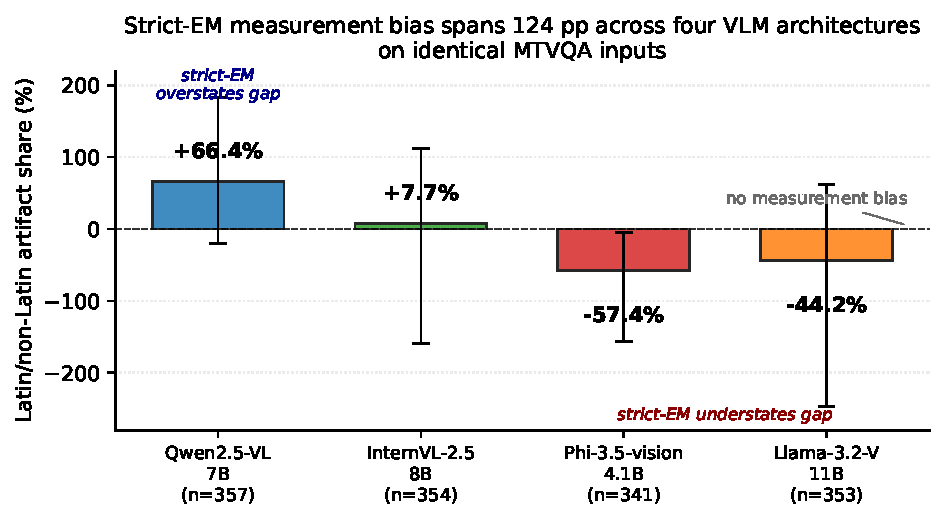
\includegraphics[width=\columnwidth]{figures/fig_four_vlm_artifact.pdf}
\caption{\textbf{Four VLM architectures, four artifact shares, 124 pp spread.} Point estimates with 95\% bootstrap CIs (2000 iterations). Qwen ($+66\%$): strict-EM overstates the Latin/non-Latin gap. InternVL ($+8\%$): approximately well-calibrated. Phi ($-57\%$, CI excludes zero) and Llama-3.2-Vision-11B ($-44\%$): strict-EM \emph{understates} the gap; both fall on the same side of zero, confirming the architecture-dependence is not a Phi-only artifact.}
\label{fig:four-vlm-artifact}
\end{figure}

\paragraph{Output-style verbosity is the mechanism.}
Qwen2.5-VL-7B is more verbose on non-Latin --- it answers a date question with a date \emph{plus context}, an address with the address \emph{plus country}, a numeric with the numeral \emph{plus unit}; each addition is correct but byte-misses gold. InternVL is terser by default and Phi shorter still; Llama-3.2-Vision is the most pronounced terse-on-non-Latin model of the four. We quantify this in Table~\ref{tab:verbosity}: the non-Latin/Latin output-length ratio broadly tracks the artifact-share rank, with the two negative-artifact-share architectures (Phi $0.62$, Llama $0.59$) having the lowest ratios. Phi's Latin outputs are nearly as long as Qwen's ($28.1$ vs $30.9$ chars) but its non-Latin outputs are the shortest of the three baselines ($17.4$ chars); on Latin it underperforms strict-EM by paraphrasing the longer gold, on non-Latin it overperforms by happening to match the short gold, yielding the negative artifact share. The pattern replicates at population: on joint $n=2142$, Qwen's ratio is $0.88$ vs InternVL's $0.66$, a $0.22$ split tracking the $+27.4$ pp artifact-share difference. Output-style verbosity is a measurable architecture-level prior, and is the largest single mechanism behind the architecture-specific strict-EM artifact share.

\begin{table}[t]
\centering
\small
\begin{tabular}{lrrrr}
\toprule
VLM & Latin & non-Latin & ratio & artifact \\
\midrule
Qwen-7B            & 30.9 & 27.8 & $0.90$ & $+66\%$ \\
InternVL-8B         & 26.6 & 18.0 & $0.68$ & $+8\%$ \\
Phi-3.5             & 28.1 & 17.4 & $0.62$ & $-57\%$ \\
Llama-3.2-V-11B    & 47.5 & 28.2 & $0.59$ & $-44\%$ \\
\bottomrule
\end{tabular}
\caption{\textbf{Mean output character count by VLM and script}, 341-row 3-VLM joint held-out for Qwen/InternVL/Phi and 355-row Llama held-out (under identical prompt). The non-Latin/Latin ratio broadly tracks artifact share: lower ratio $\Rightarrow$ more negative artifact share.}
\label{tab:verbosity}
\end{table}

\paragraph{XFUND within-CJK control.}
We replicate on XFUND (1394 rows over 7 languages). The cross-script Latin/CJK gap on XFUND is small (strict $+1.6$ pp $\to$ sem-EM $+1.1$ pp; artifact share $35\%$), but the within-CJK Japanese-vs-Chinese gap is large and \emph{survives} semantic-EM: $+29.6$ pp strict $\to +25.9$ pp sem-C, only $12\%$ artifact (Appendix~\ref{app:xfund}). This is the dual of the cross-script finding: cross-script gaps are largely artifact ($65\%$ on MTVQA), within-script CJK gaps are largely real ($88\%$ real on XFUND). Semantic-EM does not erase all cross-lingual differences; it isolates the surface-form-attributable component and leaves the genuine capability-attributable component visible.
